%% Copyright (C) 2000, 2001, 2005, 2006   Free Software Foundation
%%
%%  Verbatim copying of this entire article is permitted, provided this
%% notice is preserved.

\documentclass[twoside,12pt]{article}

%% Packages

\usepackage{url}
\usepackage{graphicx}
\usepackage{wrapfig}

%% French

\usepackage[utf8]{inputenc}
\usepackage[T1]{fontenc}
\usepackage{ae,aeguill}
\usepackage[canadian]{babel}

%% Layout

\oddsidemargin 0in
\evensidemargin 0in
\topmargin 0in
\textwidth 6.5in
\textheight 9in

\parindent 0in
\parskip 0.043in
\pagestyle{empty}

%% Document

\begin{document}

\begin{center}

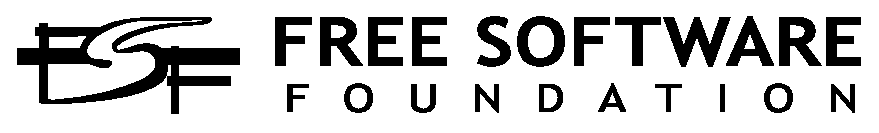
\includegraphics{fsf-logo.eps}

\vspace{0.3in}

{\Huge\bf Qu'est-ce que le logiciel libre?}

\end{center}

\begin{wrapfigure}{l}{2.0in}
 \begin{center}
   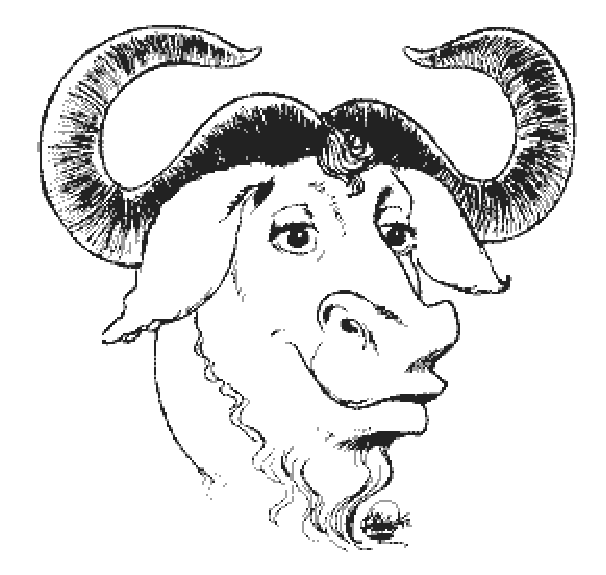
\includegraphics[width=2in]{gnu-head.eps}
 \end{center}
\end{wrapfigure}

Le logiciel libre c'est du logiciel qui respecte nos libertés. Utiliser du
logiciel libre, c'est faire le choix politique et éthique d'affirmer nos droits
et de partager ce qu'on apprend avec les autres.

%%Free software is software that respects our freedom. To use free software is to
%%make a political and ethical choice asserting our rights to learn and to share
%%what we learn with others.

Habituellement, les logiciels que nous achetons restreignent nos droits, car
nous n'achetons pas la propriété du logiciel. Ce que nous achetons c'est une
licence d'utilisation du logiciel. Cette licence nous contraint par plusieurs
règles en petits caractères stipulant ce que nous pouvons et ne pouvons pas
faire.

%%Usually software we buy denies us these rights, because we don't actually buy
%%ownership of the software. Instead, we receive a license to use the software,
%%and this license binds us with many fine-print rules about what we can and
%%can't do.

En copiant le logiciel pour le donner à un ami, en essayant d'apprendre le
fonctionnement d'un programme, en l'installant sur plus d'une de nos propres
machines, dans notre propre maison, nous sommes passibles d'une amende ou d'une
peine de prison. Voilà ce qui se trouve dans les petits caractères.

%%If we make a copy and give it to a friend, if we try to figure out how the
%%program works, if we put a copy on more than one of our own computers in our
%%own home, we could if caught be fined or put in jail. That's what's in the fine
%%print.

Que se passerait-il, si un groupe mondial de programmeurs éthiques et
talentueux dévoués à l'idée d'écrire et de partager du logiciel avec tous ceux
qui sont d'accord de le partager sous les mêmes conditions. Et qu'est-ce qui se
passerait si tout le monde pouvait faire partie et bénéficier de cette
communauté sans pour autant connaitre la programmation? Nous n'aurions plus
peur de nous faire prendre à copier un logiciel pour un ami, car ça ne serait
plus illégal.

%What if there were a worldwide group of talented ethical programmers
%voluntarily committed to the idea of writing and sharing software with each
%other and with anyone else who agreed to share alike? What if anyone could be a
%part of and benefit from this community even without knowing anything about
%programming? We wouldn't have to worry about getting caught copying a useful
%program for our friends---because we wouldn't be doing anything illegal.

\begin{wrapfigure}[14]{r}{1.5in}
 \begin{center}
   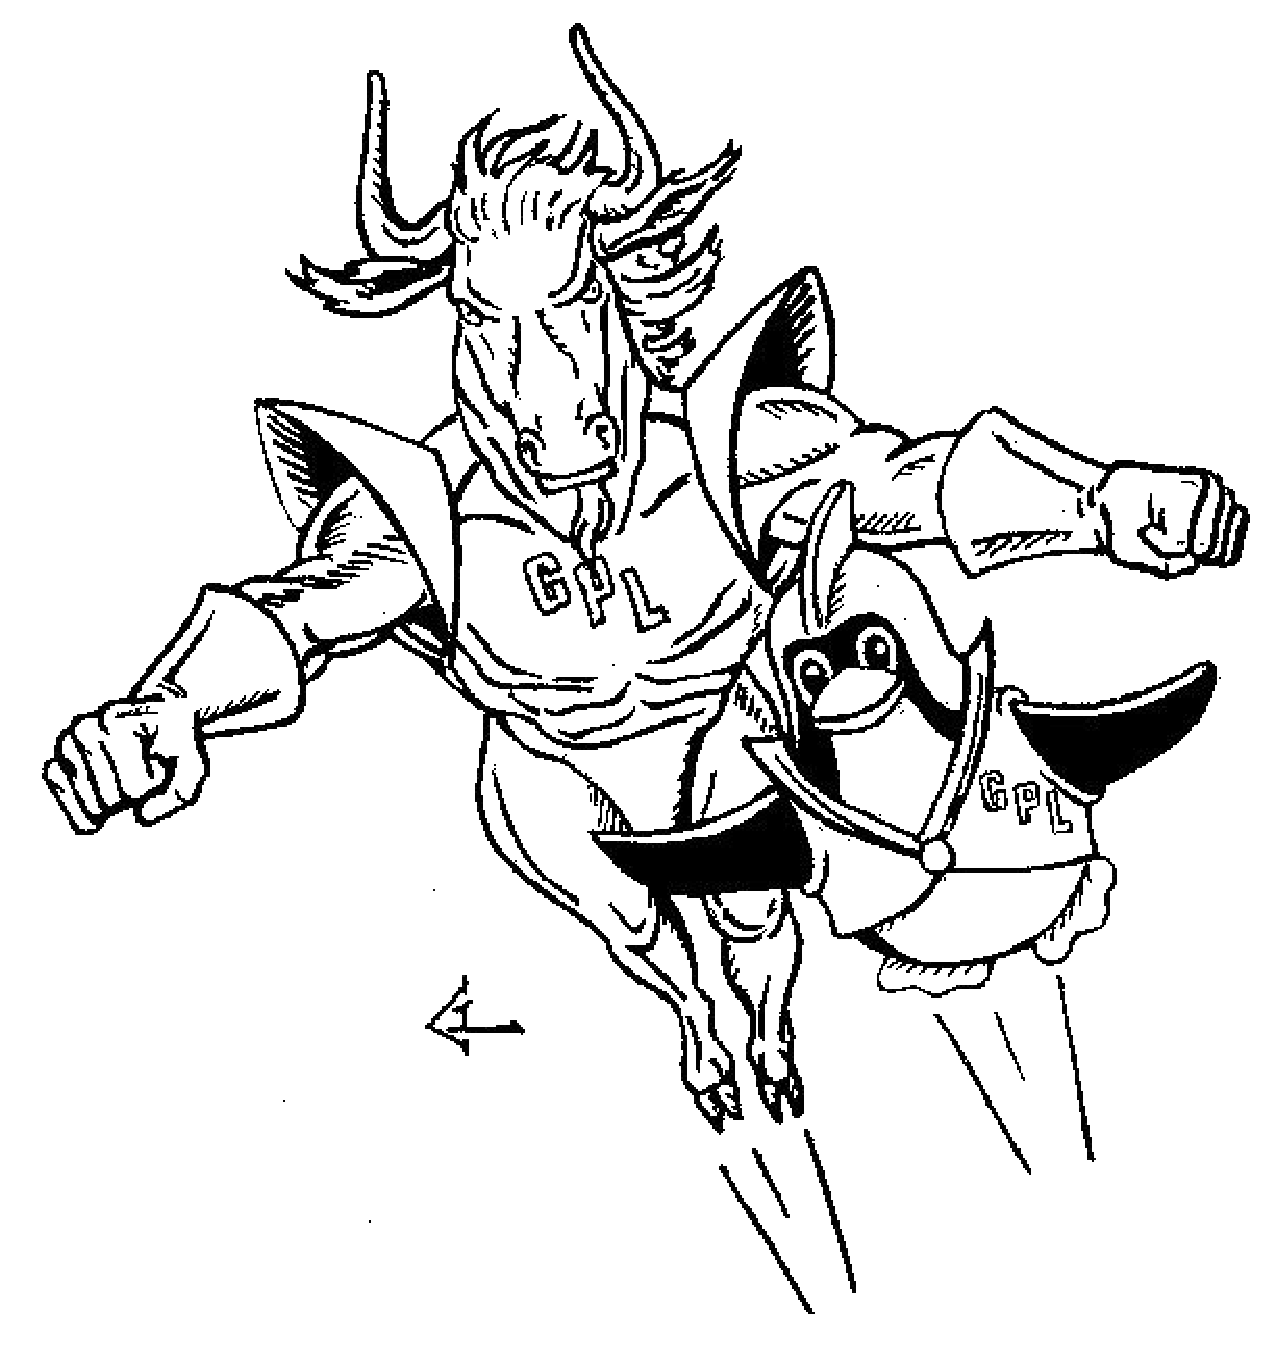
\includegraphics[scale=0.23]{dynamic-duo-bw.eps}
 \end{center}
\end{wrapfigure}

\begin{center}
{\Large\bf The Free Software Movement}
\end{center}

In fact, such a movement exists, and you can be a part of it. The free software
movement was started in 1984 by Richard M. Stallman, when he launched a project
called GNU, which stands for ``GNU's Not UNIX'', to provide a replacement for
the UNIX operating system---a replacement that would respect the freedoms of
those using it. Then in 1985, Stallman started the Free Software Foundation, a
nonprofit with the mission of advocating and educating on behalf of computer
users around the world.

Today the number of people who are not computer users is dwindling all the
time, as technology seeps around the globe. It takes knowledge to make this
technology work. People who hoard this knowledge, punishing and threatening
others who try to obtain and share it, are not doing so in order to preserve
it, despite what they may claim. Instead, they are preserving power for
themselves at the expense of others' freedom.

\begin{wrapfigure}[10]{l}{2in}
  \vspace{-0.25in}
  \begin{center}
    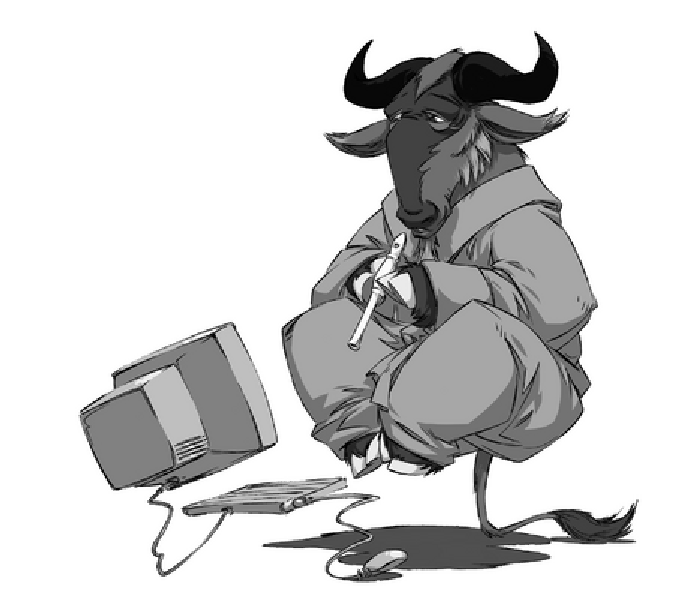
\includegraphics[scale=0.45]{gnu-think-smaller.eps}
  \end{center}
\end{wrapfigure}

%Recognizing this, millions of people around the world---including entire
%governments---have made the commitment to use only free software on their
%computers. The fact that so many people are willing to make and stand by this
%decision in the face of cheaper and cheaper ``deals'' from Microsoft, Apple and
%other proprietary software companies proves these companies wrong---we don't
%need them or their fine print to make software.

Reconnaissant cela, des millions de personnes à travers le monde---incluant des gouvernements---se sont engagés à utiliser le logiciel libre sur leurs ordinateurs. Le fait que tant de personnes soient prêtes à prendre cette décision face à des propositions de plus en plus ``abordable'' de Microsoft, Apple et d'autres compagnies de logiciels propriétaires prouve que ces compangies sont dans le tort---nous n'avons pas besoin d'eux ou de leur permission pour faire du logiciel.

%We can do it ourselves. We are doing it ourselves.

Nous pouvons le faire nous même. Nous le faisons déjà nous même.

\begin{center}
{\Large\bf How Does It Work? Copyleft!}
\end{center}

Because the copyright laws covering software are often used to take away our
freedoms, Stallman and the FSF developed a specific legal document called the
GNU General Public License (GPL) to protect them. Instead of restricting what
we can do with software the GPL encourages us to learn and share, so it is
called a ``copyleft'' license. Thousands of people and businesses---from
hobbyists to big companies like IBM and Novell---are now authoring and
distributing free software using the GPL.

But which software to use is a political choice for all of us, not just the
people who program and sell it. We can click our freedoms away by signaling
{\tt OK} in the Microsoft or Macintosh window after squinting through their
thirty pages of restrictions, or we can click {\tt CANCEL}, and see instead if
there is a piece of free software that does what we need.

We should click {\tt CANCEL} when we can because that's the more ethical choice.
This means we'll have to learn a new program, and sometimes the free program
might not work as well. The ethical choice is not always the easy choice.

\begin{center}
{\Large\bf Get Involved}
\end{center}

You can start by making a commitment to look for free software alternatives.
The Free Software Directory (\url{http://directory.fsf.org}) lists over 5,000 free
programs.

There are many other ways for people with and without programming skills to
help the free software movement continue to succeed. Please see the websites of
the Free Software Foundation (\url{http://www.fsf.org}) and the GNU project,
(\url{http://www.gnu.org}) to find out how.

And of course, please make copies of this information and share it with
others!

\vspace{0.3in}

{\small

\noindent Copyright \copyright\/ 2000, 2001, 2005, 2006 Free Software Foundation, Inc., 51
Franklin Street, 5th Floor, Boston, MA 02110, USA.

Verbatim copying and distribution of this entire article is permitted
in any medium, provided this notice is preserved.
}

\end{document}
